\clearpage
\section{Disable write-frame MISO echo: 15 November 2026}
The diagnostic parser previously connected MISO directly to the same shift
register used for MOSI reception. Consequently write transactions returned
delayed received bits despite requiring no read response. This shortcut is
unnecessary for the diagnostic protocol. The canonical parser now drives
\texttt{reading ? data[15] : 0}. SPI write commits and read replies are retained.
The output stays defined low during selected writes; FPGA Hi-Z would only
float DD29's input because the external buffer has no separate output enable.
HSEL-controlled FPGA output enable, drive strength and external clock profiles
are unchanged. This reduces unnecessary activity; it does not identify or
repair the physical reason legitimate MISO activity disturbs SYS clock lock.

Image \texttt{71ac56fb} defaults to quiet-write mode4 at CSR0x305. Mode0
restores the original echo for an in-image comparison. The raw core is retained
internally for that control; the default wrapper implements the same gating
as the canonical parser. Observer format30005 adds quiet-write enable at bit14,
while parser hold/clamp remain disabled. Simulation independently verified both
implementations, every write sample/edge, exact commits, and read0/1/2/scratch.
Dell timing passed: setup slack0.078ns, hold slack0.067ns.

\subsection{Comparison and limitations}
The first long series recorded12 quiet writes without reset and eight raw
controls, five with SYS reset, before ARM writes stopped working. It restored
c7531465 and passed original-image ADC/power/frontend checks. A shorter run
completed the following sequence using fixed qualified scratch packets:
\begin{center}\begin{tabular}{lrr}\toprule
Condition & Frames & SYS reset / LOCK losses\\\midrule
Quiet writes, first block &12&0/12\\
Raw echo, one FFFF positive control &1&1/1\\
Quiet writes, return block &12&0/12\\
Quiet-write mode: read0/1/2 &3&3/3\\\bottomrule
\end{tabular}\end{center}
All25 scratch writes committed; all three signature replies were correct.
Every sampled write MISO value in quiet mode was0. The raw positive control
is a single frame, not an estimated failure rate. The earlier partial raw
control cohort is retained separately. No SPI readback occurs in write blocks.

The three read controls still lost SYS LOCK despite correct data. The write
fix therefore does not resolve the clock fault during reads, and the board is
not unconditionally released. After that deliberate reset stress, candidate
postflight failed an assertion; the wrapper restored c7531465 and its ADC checks
passed. The failing check was not captured in sufficient detail to attribute
it to a specific frontend/register condition; it is not reported as a candidate
postflight PASS. A separate fresh-load installation run validates the final state.

\begin{center}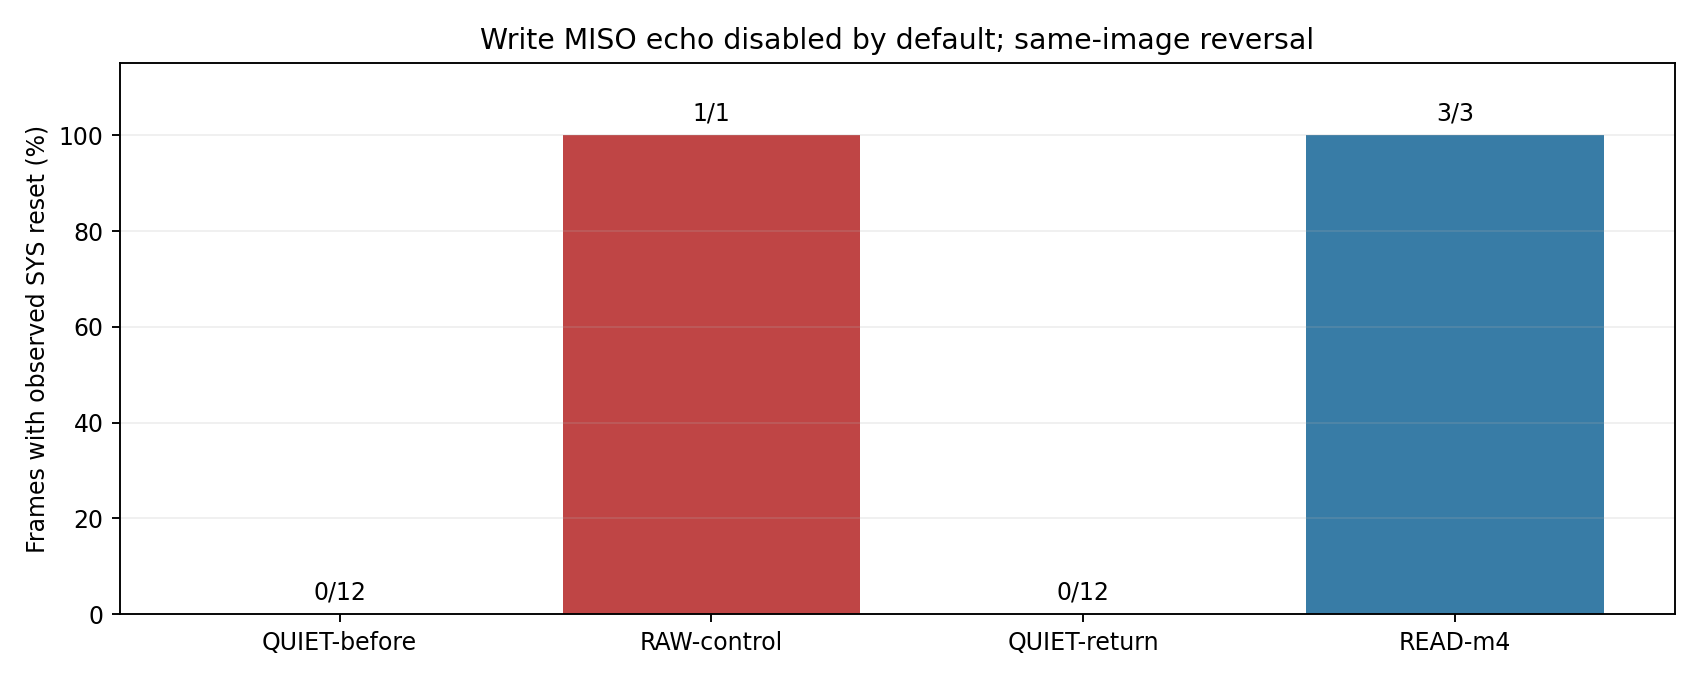
\includegraphics[width=\linewidth]{write-quiet.png}\end{center}

\subsection{Final fresh-load installation}
After reloading the identical bitstream, a separate installation run completed
another24 quiet writes, with all commits correct, no sampled MISO edges and
no SYS resets/LOCK losses. No raw/read fault controls were repeated in that
installation run. Mode305 readback was53520004, generator306 was474e0000,
frontend readiness was0xfff, power-good was healthy and all12 physical ADC
bank-A captures passed on the first attempt. The run exited0 and retained
image71ac56fb in FPGA SRAM. Configuration flash was not programmed.

Bitstream SHA256:
\begin{center}\path{0407f67e189a25bfee0f6fe02bc6d805c79eedc8b75ce1cca24d2a6dca06daf1}\end{center}
Kasli outputs stayed driven, original divider600 was restored and CFD e0
remained0. All hardware leases were released. Raw runs, source/bitstream,
separate simulations, qualified Dell reports and installation receipts:
\begin{center}\path{system/evidence-write-quiet-20261115}\end{center}
